% !TEX TS-program = pdflatex
\documentclass[11pt]{article}

% -------------------- Packages --------------------
\usepackage[a4paper,margin=1in]{geometry}
\usepackage{amsmath,amssymb}
\usepackage[T1]{fontenc}
\usepackage{lmodern}
\usepackage{xcolor}
\usepackage{tcolorbox}
\tcbuselibrary{skins,breakable}
\usepackage{enumitem}
\usepackage{hyperref}
\usepackage{tikz}
\usetikzlibrary{calc,angles,quotes}

\pagestyle{empty}

% -------------------- Dark Theme Colors --------------------
\definecolor{bg}{HTML}{000000}
\definecolor{pairbg}{HTML}{121212}
\definecolor{solbg}{HTML}{0A0A0A}
\definecolor{border}{HTML}{2A2A2A}
\definecolor{text}{HTML}{FFFFFF}
\definecolor{muted}{HTML}{C9CDD3}
\definecolor{gold}{HTML}{FFD700}
\definecolor{green}{HTML}{4ADE80}
\definecolor{cyan}{HTML}{38BDF8}

\pagecolor{bg}
\color{text}

\hypersetup{
  colorlinks=true,
  linkcolor=cyan,
  urlcolor=cyan
}

\setlength{\parindent}{0pt}
\setlength{\parskip}{10pt}

\setlist[itemize]{left=1.4em,itemsep=6pt,topsep=6pt}
\setlist[enumerate]{left=1.6em,itemsep=4pt,topsep=4pt}

% -------------------- tcolorbox Base --------------------
\tcbset{
  enhanced,
  breakable,
  arc=12pt,
  boxrule=0.8pt,
  left=16pt,right=16pt,top=12pt,bottom=12pt,
  before upper=\raggedright,
  before lower=\raggedright
}

\newtcolorbox{QAPair}[1]{%
  colback=pairbg,
  colbacklower=solbg,
  colframe=border,
  coltext=text,
  title=\textcolor{gold}{\bfseries #1},
  fonttitle=\bfseries,
  coltitle=text,
  segmentation style={draw=border, dashed, line width=0.6pt},
}

\newtcolorbox{QuickBox}{%
  colback=pairbg,
  colframe=cyan,
  coltext=text,
  fontupper=\color{text},
  borderline north={4pt}{0pt}{cyan},
  arc=14pt,
  boxrule=0.8pt
}

% Helper for step headings
\newcommand{\Step}[1]{\textcolor{muted}{\textbf{Step #1:}}}

% -------------------- TikZ styles --------------------
\tikzset{
  geom/.style={draw=text, line width=0.95pt},
  strong/.style={draw=cyan, line width=1.15pt},
  helper/.style={draw=muted, dashed, line width=0.8pt},
  lab/.style={text=text, font=\small},
  note/.style={text=muted, font=\small},
  ang/.style={draw=cyan, line width=0.95pt},
}

\newcommand{\Diag}[1]{\begin{center}#1\end{center}}

% -------------------- Diagram macros --------------------
% SAS at C (a=BC, b=CA, included angle at C is gamma) -> interior OK with A--C--B
\newcommand{\TriSASatC}[3]{%
\Diag{%
\begin{tikzpicture}[scale=0.9]
  \coordinate (C) at (0,0);
  \coordinate (A) at (4.2,0);
  \coordinate (B) at (1.3,2.7);
  \draw[geom] (A)--(B)--(C)--cycle;

  \draw[strong] (C)--(A);
  \draw[strong] (C)--(B);

  \node[lab, below] at ($(C)!0.5!(A)$) {$b=#2$};
  \node[lab, left]  at ($(C)!0.5!(B)$) {$a=#1$};
  \node[lab, above right] at ($(A)!0.5!(B)$) {$c$};

  \pic[ang, angle radius=8mm, angle eccentricity=1.25, "$\gamma=#3$"] {angle = A--C--B};

  \fill (A) circle(1.2pt) node[lab, below right] {$A$};
  \fill (B) circle(1.2pt) node[lab, above] {$B$};
  \fill (C) circle(1.2pt) node[lab, below left] {$C$};
\end{tikzpicture}}%
}

% SAS at A (b=AC, c=AB, included angle at A is alpha) -> interior OK with B--A--C
\newcommand{\TriSASatA}[3]{%
\Diag{%
\begin{tikzpicture}[scale=0.9]
  \coordinate (A) at (0,0);
  \coordinate (B) at (4.3,0.4);
  \coordinate (C) at (1.2,2.9);
  \draw[geom] (A)--(B)--(C)--cycle;

  \draw[strong] (A)--(C);
  \draw[strong] (A)--(B);

  \node[lab, left]  at ($(A)!0.5!(C)$) {$b=#1$};
  \node[lab, below] at ($(A)!0.5!(B)$) {$c=#2$};
  \node[lab, right] at ($(B)!0.5!(C)$) {$a$};

  \pic[ang, angle radius=8mm, angle eccentricity=1.25, "$\alpha=#3$"] {angle = B--A--C};

  \fill (A) circle(1.2pt) node[lab, below left] {$A$};
  \fill (B) circle(1.2pt) node[lab, below right] {$B$};
  \fill (C) circle(1.2pt) node[lab, above] {$C$};
\end{tikzpicture}}%
}

% SAS at B (c=BA, a=BC, included angle at B is beta)
% IMPORTANT FIX: use C--B--A to draw the INTERIOR angle (not reflex)
\newcommand{\TriSASatB}[3]{%
\Diag{%
\begin{tikzpicture}[scale=0.9]
  \coordinate (B) at (0,0);
  \coordinate (C) at (4.4,0);
  \coordinate (A) at (1.3,2.8);
  \draw[geom] (A)--(B)--(C)--cycle;

  \draw[strong] (B)--(A);
  \draw[strong] (B)--(C);

  \node[lab, left]  at ($(B)!0.5!(A)$) {$c=#1$};
  \node[lab, below] at ($(B)!0.5!(C)$) {$a=#2$};
  \node[lab, right] at ($(A)!0.5!(C)$) {$b$};

  % interior angle at B:
  \pic[ang, angle radius=8mm, angle eccentricity=1.25, "$\beta=#3$"] {angle = C--B--A};

  \fill (A) circle(1.2pt) node[lab, above] {$A$};
  \fill (B) circle(1.2pt) node[lab, below left] {$B$};
  \fill (C) circle(1.2pt) node[lab, below right] {$C$};
\end{tikzpicture}}%
}

% One side + two angles (generic triangle; these are already interior with this point order)
\newcommand{\TriAnglesSideA}[4]{%
\Diag{%
\begin{tikzpicture}[scale=0.9]
  \coordinate (C) at (0,0);
  \coordinate (B) at (4.6,0);
  \coordinate (A) at (1.1,2.9);
  \draw[geom] (A)--(B)--(C)--cycle;

  \draw[strong] (B)--(C);
  \node[lab, below] at ($(B)!0.5!(C)$) {$a=#1$};

  \pic[ang, angle radius=8mm, angle eccentricity=1.18, "$\alpha=#2$"] {angle = C--A--B};
  \pic[ang, angle radius=7mm, angle eccentricity=1.18, "$\beta=#3$"]  {angle = A--B--C};
  \pic[helper, angle radius=6mm, angle eccentricity=1.22, "$\gamma=#4$"] {angle = B--C--A};

  \fill (A) circle(1.2pt) node[lab, above] {$A$};
  \fill (B) circle(1.2pt) node[lab, below right] {$B$};
  \fill (C) circle(1.2pt) node[lab, below left] {$C$};
\end{tikzpicture}}%
}

\newcommand{\TriAnglesSideB}[4]{%
\Diag{%
\begin{tikzpicture}[scale=0.9]
  \coordinate (C) at (0,0);
  \coordinate (B) at (4.6,0);
  \coordinate (A) at (1.1,2.9);
  \draw[geom] (A)--(B)--(C)--cycle;

  \draw[strong] (C)--(A);
  \node[lab, left] at ($(C)!0.5!(A)$) {$b=#1$};

  \pic[ang, angle radius=8mm, angle eccentricity=1.18, "$\alpha=#2$"] {angle = C--A--B};
  \pic[ang, angle radius=7mm, angle eccentricity=1.18, "$\beta=#3$"]  {angle = A--B--C};
  \pic[helper, angle radius=6mm, angle eccentricity=1.22, "$\gamma=#4$"] {angle = B--C--A};

  \fill (A) circle(1.2pt) node[lab, above] {$A$};
  \fill (B) circle(1.2pt) node[lab, below right] {$B$};
  \fill (C) circle(1.2pt) node[lab, below left] {$C$};
\end{tikzpicture}}%
}

\newcommand{\TriAnglesSideC}[4]{%
\Diag{%
\begin{tikzpicture}[scale=0.9]
  \coordinate (C) at (0,0);
  \coordinate (B) at (4.6,0);
  \coordinate (A) at (1.1,2.9);
  \draw[geom] (A)--(B)--(C)--cycle;

  \draw[strong] (A)--(B);
  \node[lab, above right] at ($(A)!0.5!(B)$) {$c=#1$};

  \pic[ang, angle radius=8mm, angle eccentricity=1.18, "$\alpha=#2$"] {angle = C--A--B};
  \pic[ang, angle radius=7mm, angle eccentricity=1.18, "$\beta=#3$"]  {angle = A--B--C};
  \pic[helper, angle radius=6mm, angle eccentricity=1.22, "$\gamma=#4$"] {angle = B--C--A};

  \fill (A) circle(1.2pt) node[lab, above] {$A$};
  \fill (B) circle(1.2pt) node[lab, below right] {$B$};
  \fill (C) circle(1.2pt) node[lab, below left] {$C$};
\end{tikzpicture}}%
}

\newcommand{\TriSSS}[3]{%
\Diag{%
\begin{tikzpicture}[scale=0.9]
  \coordinate (C) at (0,0);
  \coordinate (B) at (4.7,0);
  \coordinate (A) at (1.4,2.8);
  \draw[geom] (A)--(B)--(C)--cycle;
  \node[lab, below] at ($(B)!0.5!(C)$) {$#1$};
  \node[lab, left]  at ($(C)!0.5!(A)$) {$#2$};
  \node[lab, right] at ($(A)!0.5!(B)$) {$#3$};
  \fill (A) circle(1.2pt) node[lab, above] {$A$};
  \fill (B) circle(1.2pt) node[lab, below right] {$B$};
  \fill (C) circle(1.2pt) node[lab, below left] {$C$};
\end{tikzpicture}}%
}

\newcommand{\InvalidTriangleSketch}{%
\Diag{%
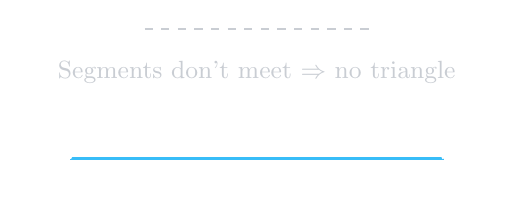
\begin{tikzpicture}[scale=0.95]
  \coordinate (L) at (0,0);
  \coordinate (R) at (5,0);
  \draw[strong] (L)--(R);
  \node[lab, below] at ($(L)!0.5!(R)$) {$c=5$};

  \coordinate (L2) at ($(L)+(60:2)$);
  \coordinate (R2) at ($(R)+(120:2)$);
  \draw[geom] (L)--(L2);
  \draw[geom] (R)--(R2);
  \node[lab, left]  at ($(L)!0.5!(L2)$) {$a=2$};
  \node[lab, right] at ($(R)!0.5!(R2)$) {$b=2$};

  \draw[helper] (L2)--(R2);
  \node[note] at (2.5,1.15) {Segments don't meet $\Rightarrow$ no triangle};
\end{tikzpicture}}%
}

% ============================================================
\begin{document}
\sloppy

\begin{center}
{\LARGE\bfseries \textcolor{gold}{Exercise 8.4 --- Solutions}}\\[-2pt]
\end{center}

% -------------------- Quick formulas + interior-angle diagram --------------------
\begin{QuickBox}
{\color{cyan}\bfseries Quick formulas (useful)}\par\medskip

\Diag{%
\begin{tikzpicture}[scale=0.85]
  \coordinate (A) at (0,2.3);
  \coordinate (B) at (4.4,0.4);
  \coordinate (C) at (0.2,0);
  \draw[geom] (A)--(B)--(C)--cycle;

  \node[lab, above] at (A) {$A$};
  \node[lab, below right] at (B) {$B$};
  \node[lab, below left] at (C) {$C$};

  \node[lab, left] at ($(A)!0.5!(C)$) {$b$};
  \node[lab, below] at ($(B)!0.5!(C)$) {$a$};
  \node[lab, right] at ($(A)!0.5!(B)$) {$c$};

  % all interior
  \pic[ang, angle radius=7mm, angle eccentricity=1.15, "$\alpha$"] {angle = C--A--B};
  \pic[ang, angle radius=6mm, angle eccentricity=1.15, "$\beta$"]  {angle = A--B--C};
  \pic[ang, angle radius=6mm, angle eccentricity=1.15, "$\gamma$"] {angle = B--C--A};

  \node[note] at (2.8,2.15) {$A_{\triangle}=\dfrac12 ab\sin\gamma$ (SAS)};
\end{tikzpicture}}%

\begin{itemize}
\item \textbf{Triangle area (two sides + included angle):}\quad
$A=\dfrac12 ab\sin\gamma=\dfrac12 bc\sin\alpha=\dfrac12 ca\sin\beta$.
\item \textbf{Triangle area (one side + two angles):}\quad
If $c$ is between angles $\alpha,\beta$ (so opposite $\gamma$), then
$A=\dfrac{c^2\sin\alpha\sin\beta}{2\sin\gamma}$.
\item \textbf{Heron's formula (three sides):}\quad
$s=\dfrac{a+b+c}{2}$,\; $A=\sqrt{s(s-a)(s-b)(s-c)}$.
\item \textbf{Parallelogram area:}\quad $A=ab\sin\theta$.
\item \textbf{Trapezoid area:}\quad $A=\dfrac12(\text{sum of parallel sides})\times h$.
\item \textbf{Minutes to degrees:}\quad $46^\circ 50' = 46+\dfrac{50}{60}^\circ$,\;
$30^\circ 15' = 30+\dfrac{15}{60}^\circ$.
\end{itemize}
\end{QuickBox}


% ---- Q1(i)
\begin{QAPair}{Question 1 (i)}
\textcolor{gold}{\bfseries Question:} $a=8,\; b=14,\; \gamma=68.7^\circ$.\par
\tcblower
\textcolor{green}{\bfseries Answer:}\par
\TriSASatC{8}{14}{68.7^\circ}
\[
A=\frac12 ab\sin\gamma=56\sin 68.7^\circ\approx 52.17.
\]
\end{QAPair}

% ---- Q1(ii)
\begin{QAPair}{Question 1 (ii)}
\textcolor{gold}{\bfseries Question:} $b=30,\; c=25,\; \alpha=46^\circ$.\par
\tcblower
\textcolor{green}{\bfseries Answer:}\par
\TriSASatA{30}{25}{46^\circ}
\[
A=\frac12 bc\sin\alpha=375\sin46^\circ\approx 269.75.
\]
\end{QAPair}

% ---- Q1(iii)
\begin{QAPair}{Question 1 (iii)}
\textcolor{gold}{\bfseries Question:} $a=20,\; c=15,\; \beta=25^\circ$.\par
\tcblower
\textcolor{green}{\bfseries Answer:}\par
\TriSASatB{15}{20}{25^\circ}
\[
A=\frac12 ac\sin\beta=150\sin25^\circ\approx 63.39.
\]
\end{QAPair}

% ---- Q1(iv)
\begin{QAPair}{Question 1 (iv)}
\textcolor{gold}{\bfseries Question:} $\beta=46^\circ 50',\; a=43,\; c=52$.\par
\tcblower
\textcolor{green}{\bfseries Answer:}\par
\TriSASatB{52}{43}{46^\circ 50'}
\[
\beta=46+\frac{50}{60}=46.8333^\circ,\quad
A=\frac12(43)(52)\sin(46.8333^\circ)\approx 815.43.
\]
\end{QAPair}

% ---- Q1(v)
\begin{QAPair}{Question 1 (v)}
\textcolor{gold}{\bfseries Question:} $b=4.5,\; c=2.5,\; \alpha=65.2^\circ$.\par
\tcblower
\textcolor{green}{\bfseries Answer:}\par
\TriSASatA{4.5}{2.5}{65.2^\circ}
\[
A=\frac12 bc\sin\alpha=5.625\sin65.2^\circ\approx 5.11.
\]
\end{QAPair}

% ---- Q1(vi)
\begin{QAPair}{Question 1 (vi)}
\textcolor{gold}{\bfseries Question:} $a=2,\; b=2,\; c=5$.\par
\tcblower
\textcolor{green}{\bfseries Answer:}\par
\InvalidTriangleSketch
\[
2+2=4<5\Rightarrow \text{no triangle is possible; area is not defined.}
\]
\end{QAPair}

% ---- Q1(vii)
\begin{QAPair}{Question 1 (vii)}
\textcolor{gold}{\bfseries Question:} $a=12,\; \alpha=44^\circ,\; \beta=60^\circ$.\par
\tcblower
\textcolor{green}{\bfseries Answer:}\par
\[
\gamma=180^\circ-44^\circ-60^\circ=76^\circ.
\]
\TriAnglesSideA{12}{44^\circ}{60^\circ}{76^\circ}
\[
A=\frac{a^2\sin\beta\sin\gamma}{2\sin\alpha}
=\frac{12^2\sin60^\circ\sin76^\circ}{2\sin44^\circ}\approx 87.10.
\]
\end{QAPair}

% ---- Q1(viii)
\begin{QAPair}{Question 1 (viii)}
\textcolor{gold}{\bfseries Question:} $b=30,\; \alpha=40^\circ,\; \beta=80^\circ$.\par
\tcblower
\textcolor{green}{\bfseries Answer:}\par
\[
\gamma=180^\circ-40^\circ-80^\circ=60^\circ.
\]
\TriAnglesSideB{30}{40^\circ}{80^\circ}{60^\circ}
\[
A=\frac{b^2\sin\alpha\sin\gamma}{2\sin\beta}\approx 254.37.
\]
\end{QAPair}

% ---- Q1(ix)
\begin{QAPair}{Question 1 (ix)}
\textcolor{gold}{\bfseries Question:} $c=10,\; \alpha=75^\circ,\; \beta=45^\circ$.\par
\tcblower
\textcolor{green}{\bfseries Answer:}\par
\[
\gamma=180^\circ-75^\circ-45^\circ=60^\circ.
\]
\TriAnglesSideC{10}{75^\circ}{45^\circ}{60^\circ}
\[
A=\frac{c^2\sin\alpha\sin\beta}{2\sin\gamma}\approx 39.43.
\]
\end{QAPair}

% ---- Q1(x)
\begin{QAPair}{Question 1 (x)}
\textcolor{gold}{\bfseries Question:} $b=21,\; \beta=30^\circ 15',\; \gamma=110^\circ$.\par
\tcblower
\textcolor{green}{\bfseries Answer:}\par
\[
\beta=30.25^\circ,\quad \alpha=180^\circ-30.25^\circ-110^\circ=39.75^\circ.
\]
\TriAnglesSideB{21}{39.75^\circ}{30.25^\circ}{110^\circ}
\[
A=\frac{b^2\sin\alpha\sin\gamma}{2\sin\beta}\approx 263.00.
\]
\end{QAPair}

% ---- Q1(xi)
\begin{QAPair}{Question 1 (xi)}
\textcolor{gold}{\bfseries Question:} $a=18.4,\; \alpha=65^\circ 10',\; \beta=95.5^\circ$.\par
\tcblower
\textcolor{green}{\bfseries Answer:}\par
\[
\alpha=65.1667^\circ,\quad \gamma=180^\circ-65.1667^\circ-95.5^\circ=19.3333^\circ.
\]
\TriAnglesSideA{18.4}{65.1667^\circ}{95.5^\circ}{19.3333^\circ}
\[
A=\frac{a^2\sin\beta\sin\gamma}{2\sin\alpha}\approx 61.47.
\]
\end{QAPair}

% ---- Q1(xii)
\begin{QAPair}{Question 1 (xii)}
\textcolor{gold}{\bfseries Question:} $c=25,\; \alpha=52.7^\circ,\; \gamma=79^\circ 24'$.\par
\tcblower
\textcolor{green}{\bfseries Answer:}\par
\[
\gamma=79.4^\circ,\quad \beta=180^\circ-52.7^\circ-79.4^\circ=47.9^\circ.
\]
\TriAnglesSideC{25}{52.7^\circ}{47.9^\circ}{79.4^\circ}
\[
A=\frac{c^2\sin\alpha\sin\beta}{2\sin\gamma}\approx 187.65.
\]
\end{QAPair}

% ---- Q1(xiii)
\begin{QAPair}{Question 1 (xiii)}
\textcolor{gold}{\bfseries Question:} sides $18,\;21,\;32$.\par
\tcblower
\textcolor{green}{\bfseries Answer:}\par
\TriSSS{18}{21}{32}
\[
s=\frac{18+21+32}{2}=35.5,\quad
A=\sqrt{35.5(17.5)(14.5)(3.5)}\approx 177.56.
\]
\end{QAPair}

% ---- Q1(xiv)
\begin{QAPair}{Question 1 (xiv)}
\textcolor{gold}{\bfseries Question:} sides $20,\;26,\;37$.\par
\tcblower
\textcolor{green}{\bfseries Answer:}\par
\TriSSS{20}{26}{37}
\[
s=41.5,\quad
A=\sqrt{41.5(21.5)(15.5)(4.5)}\approx 249.47.
\]
\end{QAPair}

% ---- Q1(xv)
\begin{QAPair}{Question 1 (xv)}
\textcolor{gold}{\bfseries Question:} sides $\dfrac12,\;\dfrac13,\;\dfrac14$.\par
\tcblower
\textcolor{green}{\bfseries Answer:}\par
\TriSSS{\frac12}{\frac13}{\frac14}
\[
s=\frac{13}{24},\quad
A=\sqrt{\frac{13}{24}\cdot\frac{1}{24}\cdot\frac{5}{24}\cdot\frac{7}{24}}
=\frac{\sqrt{455}}{576}\approx 0.0370.
\]
\end{QAPair}

% ---- Q1(xvi)
\begin{QAPair}{Question 1 (xvi)}
\textcolor{gold}{\bfseries Question:} sides $12.4,\;13.7,\;20.2$.\par
\tcblower
\textcolor{green}{\bfseries Answer:}\par
\TriSSS{12.4}{13.7}{20.2}
\[
s=23.15,\quad
A=\sqrt{23.15(10.75)(9.45)(2.95)}\approx 83.29.
\]
\end{QAPair}

% ---- Q1(xvii)
\begin{QAPair}{Question 1 (xvii)}
\textcolor{gold}{\bfseries Question:} sides $1.6,\;2.6,\;4.1$.\par
\tcblower
\textcolor{green}{\bfseries Answer:}\par
\TriSSS{1.6}{2.6}{4.1}
\[
s=4.15,\quad
A=\sqrt{4.15(2.55)(1.55)(0.05)}\approx 0.91.
\]
\end{QAPair}

% ============================================================
\begin{QAPair}{Question 2}
\textcolor{gold}{\bfseries Question:} Adjacent sides of a parallelogram are $12$ and $16$, and one interior angle is $135^\circ$. Find its area.\\
\tcblower
\textcolor{green}{\bfseries Answer:}\par

% FIX: choose points so the interior angle is clearly 135°, and draw it as interior
\Diag{%
\begin{tikzpicture}[scale=0.9]
  \coordinate (B) at (0,0);
  \coordinate (A) at (-4,0);
  \coordinate (C) at (2,2);     % 45° from B
  \coordinate (D) at ($(A)+(C)-(B)$);

  \draw[geom] (A)--(B)--(C)--(D)--cycle;

  \node[lab, below] at ($(A)!0.5!(B)$) {$16$};
  \node[lab, right] at ($(B)!0.5!(C)$) {$12$};

  % interior 135° at B: from BC to BA is 135°
  \pic[ang, angle radius=10mm, angle eccentricity=1.2, "$135^\circ$"] {angle = C--B--A};

  \fill (A) circle(1.2pt) node[lab, below left] {$A$};
  \fill (B) circle(1.2pt) node[lab, below] {$B$};
  \fill (C) circle(1.2pt) node[lab, above right] {$C$};
  \fill (D) circle(1.2pt) node[lab, above left] {$D$};
\end{tikzpicture}
}

\[
A=ab\sin\theta=(12)(16)\sin135^\circ=192\cdot\frac{\sqrt2}{2}=96\sqrt2\approx135.76.
\]
\end{QAPair}

% ============================================================
\begin{QAPair}{Question 3}
\textcolor{gold}{\bfseries Question:} Distances between the intersections are $30$ m, $34$ m, and $27$ m. Find the area of the triangular park.\\
\tcblower
\textcolor{green}{\bfseries Answer:}\par
\TriSSS{30\,m}{34\,m}{27\,m}
\[
s=45.5,\quad
A=\sqrt{45.5(15.5)(11.5)(18.5)}\approx 387.35\ \text{m}^2.
\]
\end{QAPair}

% ============================================================
\begin{QAPair}{Question 4}
\textcolor{gold}{\bfseries Question:} A field is a parallelogram with adjacent sides $2$ km and $3$ km, and the shorter diagonal is $3$ km.\\
(a) Find $\cos$ of the acute angle. (b) Find exact $\sin$ of the acute angle. (c) Find exact area. (d) Find area to nearest integer.\\
\tcblower
\textcolor{green}{\bfseries Answer:}\par

% FIX: show the ACUTE angle at A (inside), not the obtuse at B
\Diag{%
\begin{tikzpicture}[scale=0.9]
\coordinate (A) at (0,0);
\coordinate (B) at (4,0);
\coordinate (D) at (1.4,2.1);
\coordinate (C) at ($(B)+(D)-(A)$);

\draw[geom] (A)--(B)--(C)--(D)--cycle;
\draw[helper] (A)--(C); % one diagonal (for reference)

\node[lab, below] at ($(A)!0.5!(B)$) {$3$ km};
\node[lab, left]  at ($(A)!0.5!(D)$) {$2$ km};
\node[note, align=center] at (3.6,2.35) {shorter diagonal\\$=3$ km};

% acute interior angle at A between AB and AD
\pic[ang, angle radius=8mm, angle eccentricity=1.25, "$\theta$"] {angle = B--A--D};

\fill (A) circle(1.2pt) node[lab, below left] {$A$};
\fill (B) circle(1.2pt) node[lab, below] {$B$};
\fill (C) circle(1.2pt) node[lab, above right] {$C$};
\fill (D) circle(1.2pt) node[lab, above left] {$D$};
\end{tikzpicture}
}

Let the acute included angle be $\theta$ between sides $2$ and $3$.
\[
\begin{aligned}
\Step{1}\;& 3^2=2^2+3^2-2(2)(3)\cos\theta\\
& 9=13-12\cos\theta\Rightarrow \cos\theta=\frac13.\\
\Step{2}\;& \sin\theta=\sqrt{1-\frac{1}{9}}=\frac{2\sqrt2}{3}.\\
\Step{3}\;& \text{Area}=ab\sin\theta=2\cdot3\cdot\frac{2\sqrt2}{3}=4\sqrt2\ \text{km}^2.\\
\Step{4}\;& 4\sqrt2\approx 5.66\Rightarrow \text{nearest integer }=6\ \text{km}^2.
\end{aligned}
\]
\end{QAPair}

% ============================================================
\begin{QAPair}{Question 5}
\textcolor{gold}{\bfseries Question:} The roof consists of four congruent isosceles triangles. Each equal side is $22.0$ ft and the vertex angle is $75^\circ$. Find the area of one triangular section.\\
\tcblower
\textcolor{green}{\bfseries Answer:}\par

\Diag{%
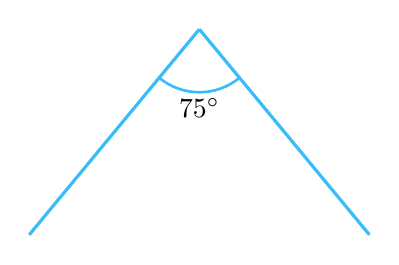
\begin{tikzpicture}[scale=0.9]
  \coordinate (V) at (0,2.9);
  \coordinate (L) at (-2.4,0);
  \coordinate (R) at (2.4,0);
  \draw[geom] (L)--(V)--(R)--cycle;

  \draw[strong] (V)--(L);
  \draw[strong] (V)--(R);

  \node[lab, left] at ($(V)!0.5!(L)$) {$22$};
  \node[lab, right] at ($(V)!0.5!(R)$) {$22$};

  \pic[ang, angle radius=8mm, angle eccentricity=1.25, "$75^\circ$"] {angle = L--V--R};
\end{tikzpicture}
}

\[
A=\frac12(22)(22)\sin75^\circ
=242\sin75^\circ
=\frac{121}{2}\sqrt2(\sqrt3+1)\approx 233.75\ \text{ft}^2.
\]
\end{QAPair}

% ============================================================
\begin{QAPair}{Question 6}
\textcolor{gold}{\bfseries Question:} An isosceles trapezoid has parallel sides $30$ ft and $20$ ft, and the other two sides are $10$ ft each. If a base angle is $60^\circ$, find the exact area.\\
\tcblower
\textcolor{green}{\bfseries Answer:}\par

\Diag{%
\begin{tikzpicture}[scale=0.82]
\coordinate (A) at (0,0);
\coordinate (B) at (6,0);
\coordinate (D) at (1,2.6);
\coordinate (C) at (5,2.6);
\draw[geom] (A)--(B)--(C)--(D)--cycle;
\node[lab, below] at ($(A)!0.5!(B)$) {$30$};
\node[lab, above] at ($(D)!0.5!(C)$) {$20$};
\node[lab, left] at ($(A)!0.5!(D)$) {$10$};
\node[lab, right] at ($(B)!0.5!(C)$) {$10$};
\draw[helper] (D)--($(A)+(1,0)$);
\draw[helper] (C)--($(B)+(-1,0)$);
\node[lab] at (1.05,1.25) {$h$};
\end{tikzpicture}
}

\[
30-20=10\Rightarrow \text{each offset}=5,\quad
h=10\sin60^\circ=5\sqrt3,\quad
A=\tfrac12(30+20)h=125\sqrt3.
\]
\end{QAPair}

% ============================================================
\begin{QAPair}{Question 7}
\textcolor{gold}{\bfseries Question:} In $\triangle ABC$, $\angle B=30^\circ$ and in $\triangle DEF$, $\angle E=150^\circ$. Show that if $AB=DE$ and $BC=EF$, then the areas are equal.\\
\tcblower
\textcolor{green}{\bfseries Answer:}\par
\[
[\triangle ABC]=\frac12(AB)(BC)\sin30^\circ=\frac{AB\cdot BC}{4},\quad
[\triangle DEF]=\frac12(DE)(EF)\sin150^\circ=\frac{DE\cdot EF}{4}.
\]
Since $AB=DE$ and $BC=EF$, the areas are equal.
\end{QAPair}

% ============================================================
\begin{QAPair}{Question 8}
\textcolor{gold}{\bfseries Question:} Area of a triangular garden is $150\text{ m}^2$. Two corner angles of a side are $40^\circ$ and $65^\circ$. Find the length of that side and the third angle.\\
\tcblower
\textcolor{green}{\bfseries Answer:}\par
\[
\gamma=180^\circ-40^\circ-65^\circ=75^\circ,\quad
150=\frac{c^2\sin40^\circ\sin65^\circ}{2\sin75^\circ}
\Rightarrow
c\approx 22.30\text{ m}.
\]
\end{QAPair}

% ============================================================
\begin{QAPair}{Question 9}
\textcolor{gold}{\bfseries Question:} An equilateral triangle is inscribed in a circle of radius $6$ cm. Find the area of the triangle.\\
\tcblower
\textcolor{green}{\bfseries Answer:}\par
\[
R=\frac{s}{\sqrt3}\Rightarrow s=6\sqrt3,\quad
A=\frac{\sqrt3}{4}s^2=27\sqrt3\ \text{cm}^2.
\]
\end{QAPair}

% ============================================================
\begin{QAPair}{Question 10}
\textcolor{gold}{\bfseries Question:} Triangle $ABC$ with $AB=15$ cm, $BC=8$ cm, and area $40$ cm$^2$.\\
(a) Find $\sin\angle B$. (b) Find $\angle B$.\\
\tcblower
\textcolor{green}{\bfseries Answer:}\par

% FIX: draw angle B INSIDE triangle (use C--B--A for this coordinate setup)
\Diag{%
\begin{tikzpicture}[scale=0.88]
\coordinate (B) at (0,0);
\coordinate (A) at (-3,0);
\coordinate (C) at (1.2,2.0);
\draw[geom] (A)--(B)--(C)--cycle;
\node[lab, below] at ($(A)!0.5!(B)$) {$AB=15$};
\node[lab, right] at ($(B)!0.5!(C)$) {$BC=8$};
\pic[ang, angle radius=7mm, angle eccentricity=1.25, "$\angle B$"] {angle = C--B--A};
\end{tikzpicture}
}

\[
40=\frac12(15)(8)\sin B=60\sin B\Rightarrow \sin B=\frac23,
\quad B\approx 41.81^\circ \text{ or } 138.19^\circ.
\]
\end{QAPair}

% ============================================================
\begin{QAPair}{Question 11}
\textcolor{gold}{\bfseries Question:} Parallelogram $ABCD$ with $AB=c$, $BC=a$, and $\angle B=\theta$.\\
(a) Write area in terms of $c,a,\theta$. (b) For what $\theta$ is the area greatest?\\
\tcblower
\textcolor{green}{\bfseries Answer:}\par

% FIX: angle at B shown as INTERIOR using C--B--A (not reflex)
\Diag{%
\begin{tikzpicture}[scale=0.88]
\coordinate (B) at (0,0);
\coordinate (A) at (-3,0);
\coordinate (C) at (1.4,2.2);
\coordinate (D) at ($(A)+(C)-(B)$);
\draw[geom] (A)--(B)--(C)--(D)--cycle;
\node[lab, below] at ($(A)!0.5!(B)$) {$c$};
\node[lab, right] at ($(B)!0.5!(C)$) {$a$};
\pic[ang, angle radius=8mm, angle eccentricity=1.25, "$\theta$"] {angle = C--B--A};
\end{tikzpicture}
}

\[
\text{Area}=ac\sin\theta,\qquad
\text{maximum when }\sin\theta=1 \Rightarrow \theta=90^\circ.
\]
\end{QAPair}

\end{document}
